\documentclass[t]{beamer}
\usetheme{Copenhagen}
\setbeamertemplate{headline}{} % remove toc from headers
\beamertemplatenavigationsymbolsempty

\usepackage{amsmath, array, tikz, bm, pgfplots, tcolorbox, graphicx, venndiagram, color, colortbl, xfrac}
\pgfplotsset{compat = 1.16}
\usepgfplotslibrary{statistics}
\usetikzlibrary{calc}

\title{Hypothesis Testing}
\subtitle{Single Sample Proportion}
\author{}
\date{}

\AtBeginSection[]
{
  \begin{frame}
    \frametitle{Objectives}
    \tableofcontents[currentsection]
  \end{frame}
}

\begin{document}

\pgfmathdeclarefunction{gauss}{2}{%
  \pgfmathparse{1/(#2*sqrt(2*pi))*exp(-((x-#1)^2)/(2*#2^2))}%
}

\begin{frame} 
\maketitle
\end{frame}

\begin{frame}{Testing a Population Proportion}
In this section, we will test a claim regarding a population proportion. \newline\\ \pause

The sample proportion, $\hat{p}$ is given by	\bigskip
\[\hat{p} = \frac{x}{n} = \frac{\text{number of observed successes}}{\text{sample size}}\]		\newline\\	\pause
with sample standard error	
\[\sigma_{\hat{p}} = \sqrt{\frac{\hat{p}(1-\hat{p})}{n}}\]
\end{frame}

\begin{frame}{Test Statistic and Critical Value Method}
The test statistic of the population proportion, $z$, can be found by calculating
\begin{align*}
z &= \frac{\hat{p} - p}{\sqrt{p(1-p)/n}} \\[10pt]
\onslide<2->{&= \frac{\text{sample proportion}-\text{population proportion}}{\text{standard error}}} \\
\end{align*}
\begin{center}
\onslide<3->{
\begin{tabular}{c|c}
\textbf{Significance Level} & \textbf{Critical Value} \\ \hline
$\alpha = 0.01$ & $\pm 2.576$ \\
$\alpha = 0.05$ & $\pm 1.96$  \\
$\alpha = 0.10$ & $\pm 1.645$ \\
\end{tabular}
}
\end{center}
\end{frame}

\begin{frame}{Test Statistic and Critical Value Method}
\begin{center}
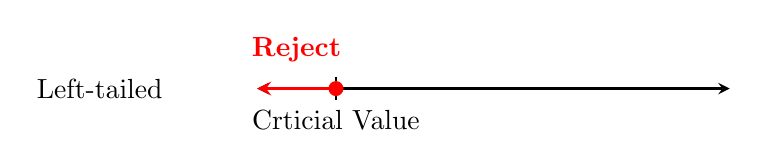
\begin{tikzpicture}[>=stealth]
\node at (-5,0) {Left-tailed};
\draw[<->, thick] (-3,0) -- (3,0);
\draw (-2,0.15) -- (-2,-0.15) node [below] {Crticial Value};
\draw [color=red, fill=red] (-2,0) circle [radius=2.5pt];
\draw[->, color=red, very thick] (-2,0) -- (-3,0);
\node at (-2.5,0.5) [color=red] {\textbf{Reject}};
\end{tikzpicture}
\newline\\
\onslide<2->{
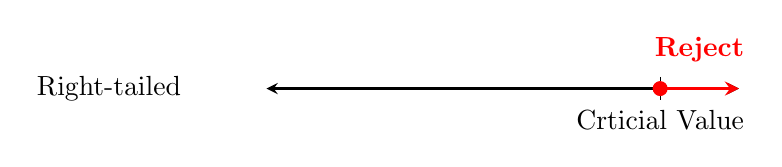
\begin{tikzpicture}[>=stealth]
\node at (-5,0) {Right-tailed};
\draw[<->, thick] (-3,0) -- (3,0);
\draw (2,0.15) -- (2,-0.15) node [below] {Crticial Value};
\draw [color=red, fill=red] (2,0) circle [radius=2.5pt];
\draw[->, color=red, very thick] (2,0) -- (3,0);
\node at (2.5,0.5) [color=red] {\textbf{Reject}};
\end{tikzpicture}}
\newline\\
\onslide<3->{
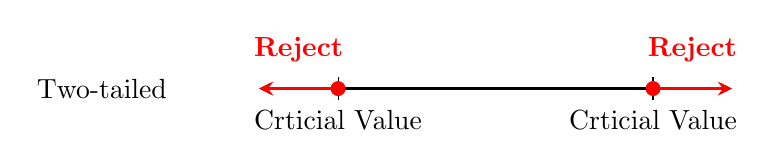
\begin{tikzpicture}[>=stealth]
\node at (-5,0) {Two-tailed};
\draw[<->, thick] (-3,0) -- (3,0);
\draw (-2,0.15) -- (-2,-0.15) node [below] {Crticial Value};
\draw [color=red, fill=red] (-2,0) circle [radius=2.5pt];
\draw[->, color=red, very thick] (-2,0) -- (-3,0);
\node at (-2.5,0.5) [color=red] {\textbf{Reject}};
\draw (2,0.15) -- (2,-0.15) node [below] {Crticial Value};
\draw [color=red, fill=red] (2,0) circle [radius=2.5pt];
\draw[->, color=red, very thick] (2,0) -- (3,0);
\node at (2.5,0.5) [color=red] {\textbf{Reject}};
\end{tikzpicture}}
\end{center}
\end{frame}

\begin{frame}{$p$-Value Method}
The area of the rejection region is given by $\alpha$, the significance level. \newline\\	\pause

Recall that the $p$-value is the probability of obtaining sample results as extreme (or more) than one we got. \newline\\	\pause

If our $p$-value is lower than $\alpha$, then our results are {\color{blue}\textbf{statistically significant}}, and would not likely occur by chance if the null hypothesis were true.	\newline\\	\pause

Reminder, if the $p\text{-value} < \alpha$, we reject the null hypothesis.
\end{frame}

\begin{frame}{$p$-Value Method}
\begin{center}
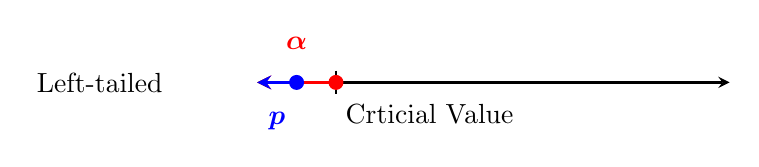
\begin{tikzpicture}[>=stealth]
\node at (-5,0) {Left-tailed};
\draw[<->, thick] (-3,0) -- (3,0);
\draw (-2,0.15) -- (-2,-0.15) node [below right] {Crticial Value};
\draw [color=red, fill=red] (-2,0) circle [radius=2.5pt];
\draw[->, color=red, very thick] (-2,0) -- (-3,0);
\node at (-2.5,0.5) [color=red] {$\bm{\alpha}$};
\onslide<2->{
\draw [color=blue, fill=blue] (-2.5,0) circle [radius=2.5pt];
\draw[->, color=blue, very thick] (-2.5,0) -- (-3,0);
\node at (-2.75,-0.25) [below, color=blue] {$\bm{p}$};
}
\end{tikzpicture}
\newline\\
\onslide<3->{\textbf{Reject null}}	\vspace{1cm}
\onslide<4->{
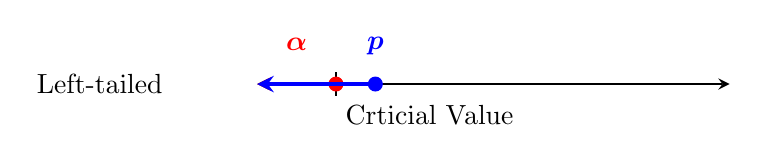
\begin{tikzpicture}[>=stealth]
\node at (-5,0) {Left-tailed};
\draw[<->, thick] (-3,0) -- (3,0);
\draw (-2,0.15) -- (-2,-0.15) node [below right] {Crticial Value};
\draw [color=red, fill=red] (-2,0) circle [radius=2.5pt];
\draw[->, color=red, very thick] (-2,0) -- (-3,0);
\node at (-2.5,0.5) [color=red] {$\bm{\alpha}$};
\onslide<5->{
\draw[->, color=blue, ultra thick] (-1.5,0) -- (-3,0);
\draw [color=blue, fill=blue] (-1.5,0) circle [radius=2.5pt];
\node at (-1.5,0.25) [above, color=blue] {$\bm{p}$};
}
\end{tikzpicture}}
\newline\\
\onslide<6->{\textbf{Do Not Reject Null}}
\end{center}
\end{frame}

\begin{frame}{Confidence Interval Method}
\begin{center}
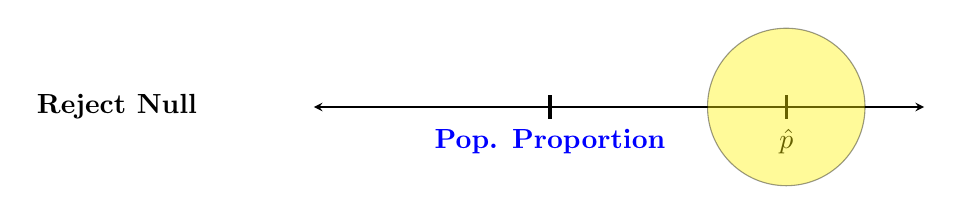
\begin{tikzpicture}[>=stealth]
\node at (-6.5,0) {\textbf{Reject Null}};
\draw[<->] (-4,0) -- (3.75,0);
\draw [very thick] (-1,0.15) -- (-1,-0.15) node [below, color=blue] {\textbf{Pop. Proportion}};
\draw [very thick] (2,0.15) -- (2,-0.15) node [below] {$\hat{p}$};
\draw [fill=yellow, opacity = 0.4] (2,0) circle [radius = 1cm];
\end{tikzpicture}
\newline\\
\onslide<2->{
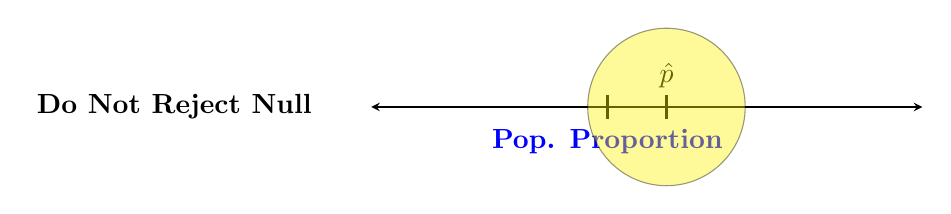
\begin{tikzpicture}[>=stealth]
\node at (-6.5,0) {\textbf{Do Not Reject Null}};
\draw[<->] (-4,0) -- (3,0);
\draw [very thick] (-1,0.15) -- (-1,-0.15) node [below, color=blue] {\textbf{Pop. Proportion}};
\draw [very thick] (-0.25,0.15) -- (-0.25,-0.15) node [above, yshift=0.25cm] {$\hat{p}$};
\draw [fill=yellow, opacity = 0.4] (-0.25,0) circle [radius = 1cm];
\end{tikzpicture}
}
\end{center}
\end{frame}

\end{document}